
\section{Signalverlauf bei Belastungen}
\noindent Die Messungen aus dem vorangegangenen Bericht vom 24.07.2023 wurden mit den fertigen Sensoren (abgeglichen und vergossen) wiederholt. Die Ergebnisse sind in Abbildung \ref{fig:vergleichlastverlauf} visualisiert
\begin{figure}[H]
	\centering
	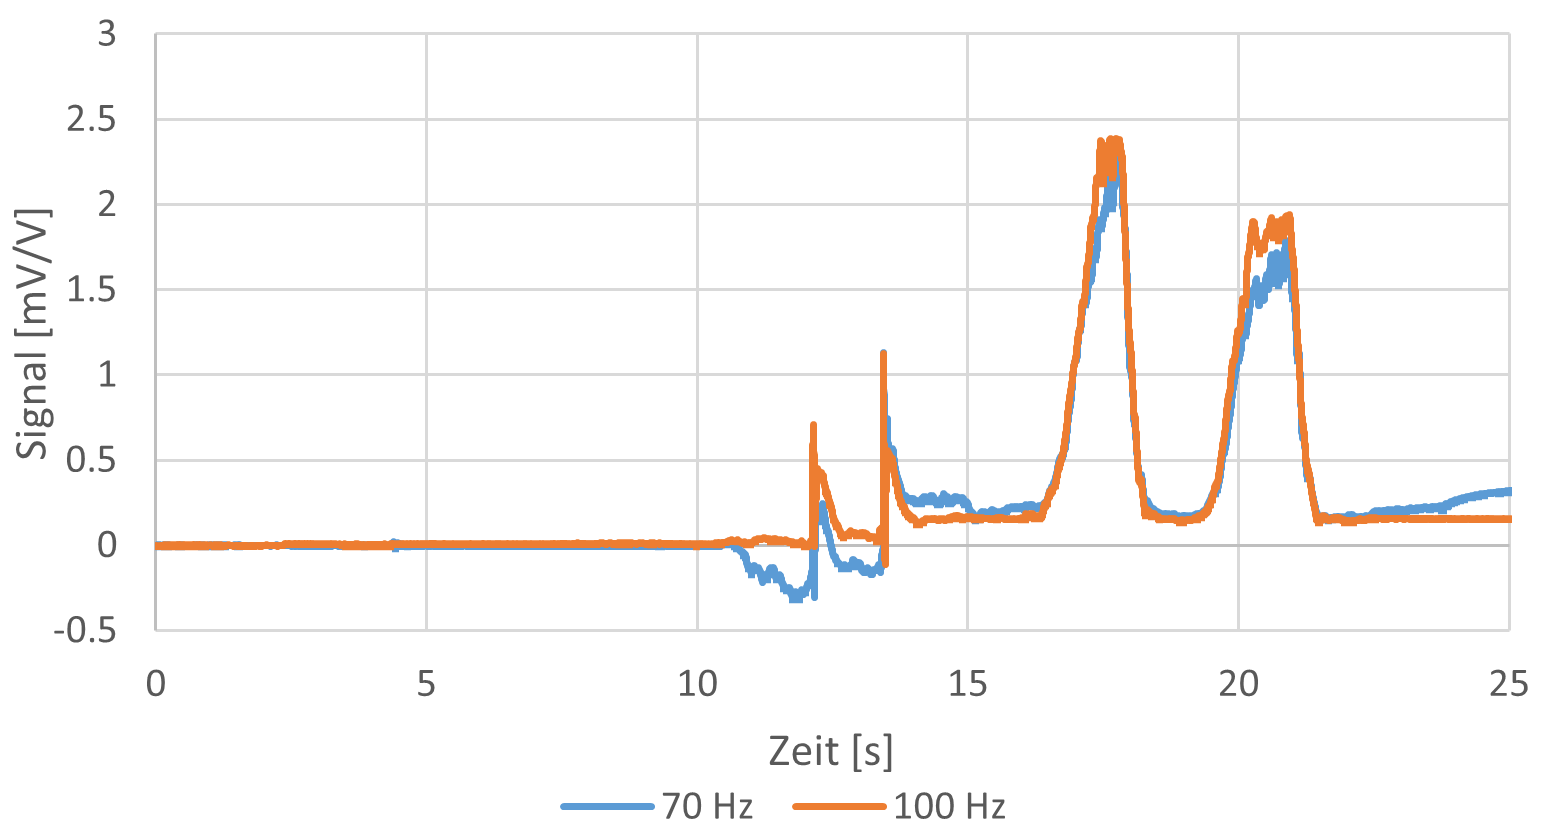
\includegraphics[width=1\linewidth]{imgs/Vergleich_Lastverlauf}
	\caption{Lastverlauf}
	\label{fig:vergleichlastverlauf}
\end{figure}
\noindent
Es fällt auf, dass die Sensoren ab der ersten Belastung (nach rund 10 Sekunden) ein schlechtes Return-to-zero-Verhalten aufweisen. Bereits nach den geringen anfänglichen Belastungen von 0.5 ... 1 mV/V weicht weichen beide Sensoren um rund 0.1 mV/V vom eigentlichen Nullpunkt ab. Dieses Verhalten konnte bei den Messungen vor Abgleich \& Verguss nicht festgestellt werden. Das Ergebniss des unvergossenen Sensors mit 100Hz Eckfrequenz ist zum Vergleich in der Abbildung \ref{fig:dutsolounvergossen} nochmal dargestellt.
\begin{figure}[H]
	\centering
	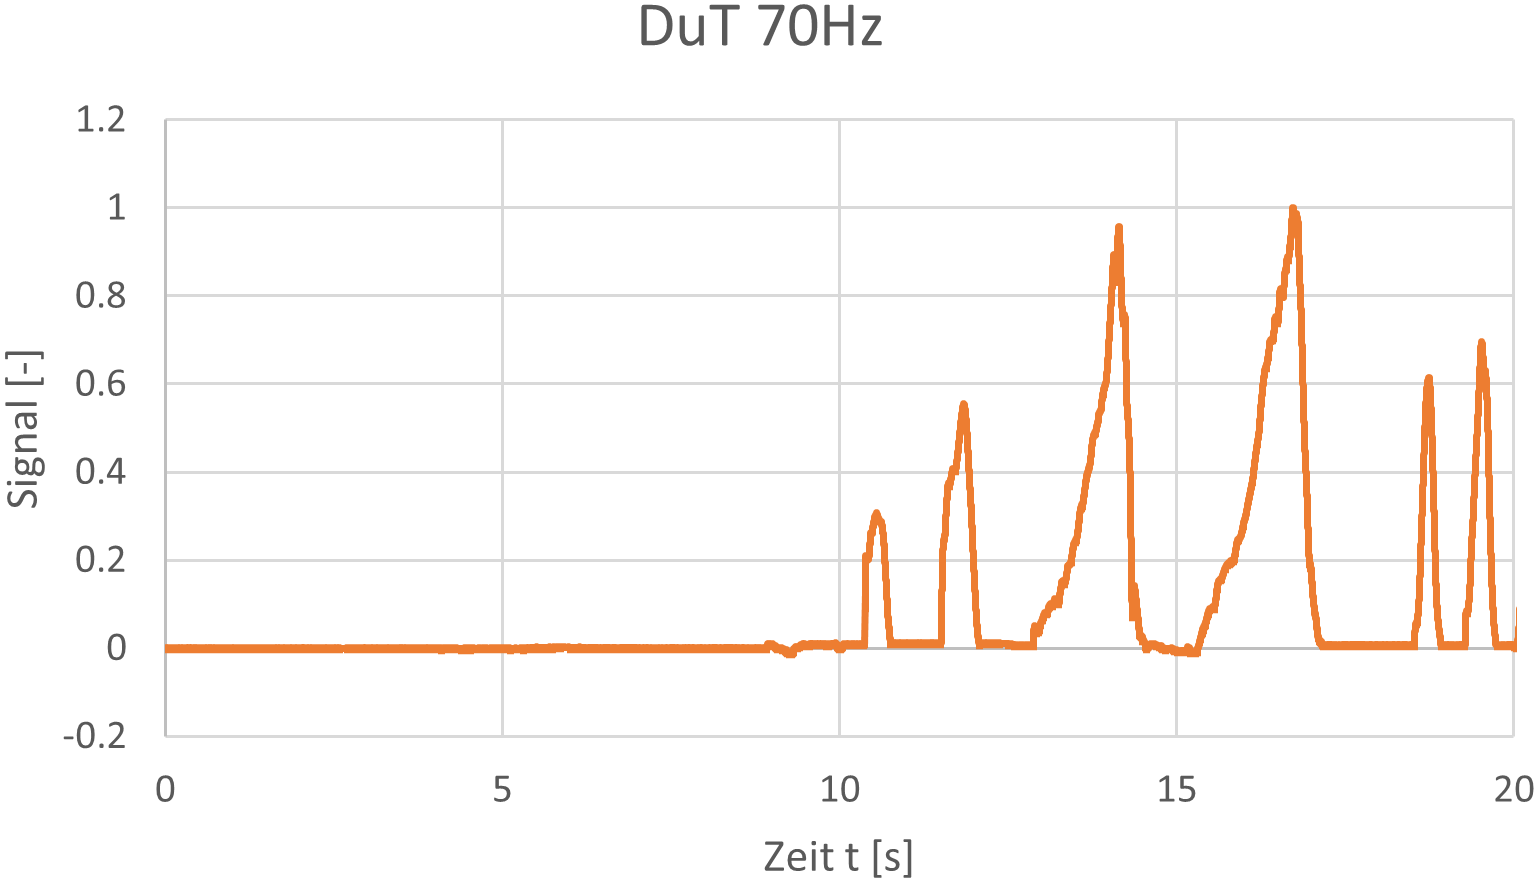
\includegraphics[width=1\linewidth]{imgs/dut_solo_unvergossen}
	\caption{DuT 70 Hz vor Verguss und Abbgleich}
	\label{fig:dutsolounvergossen}
\end{figure}
\section{Fourier-Analyse NP-Signale}
In den folgenden zwei Abbildungen sind die Frequenzspektren der Nullpunktsignal der beiden DuTs visualisiert. In der Abbildung \ref{fig:fftvergleich} sind die Spektren im Vergleich zu sehen.
\begin{figure}[H]
	\centering
	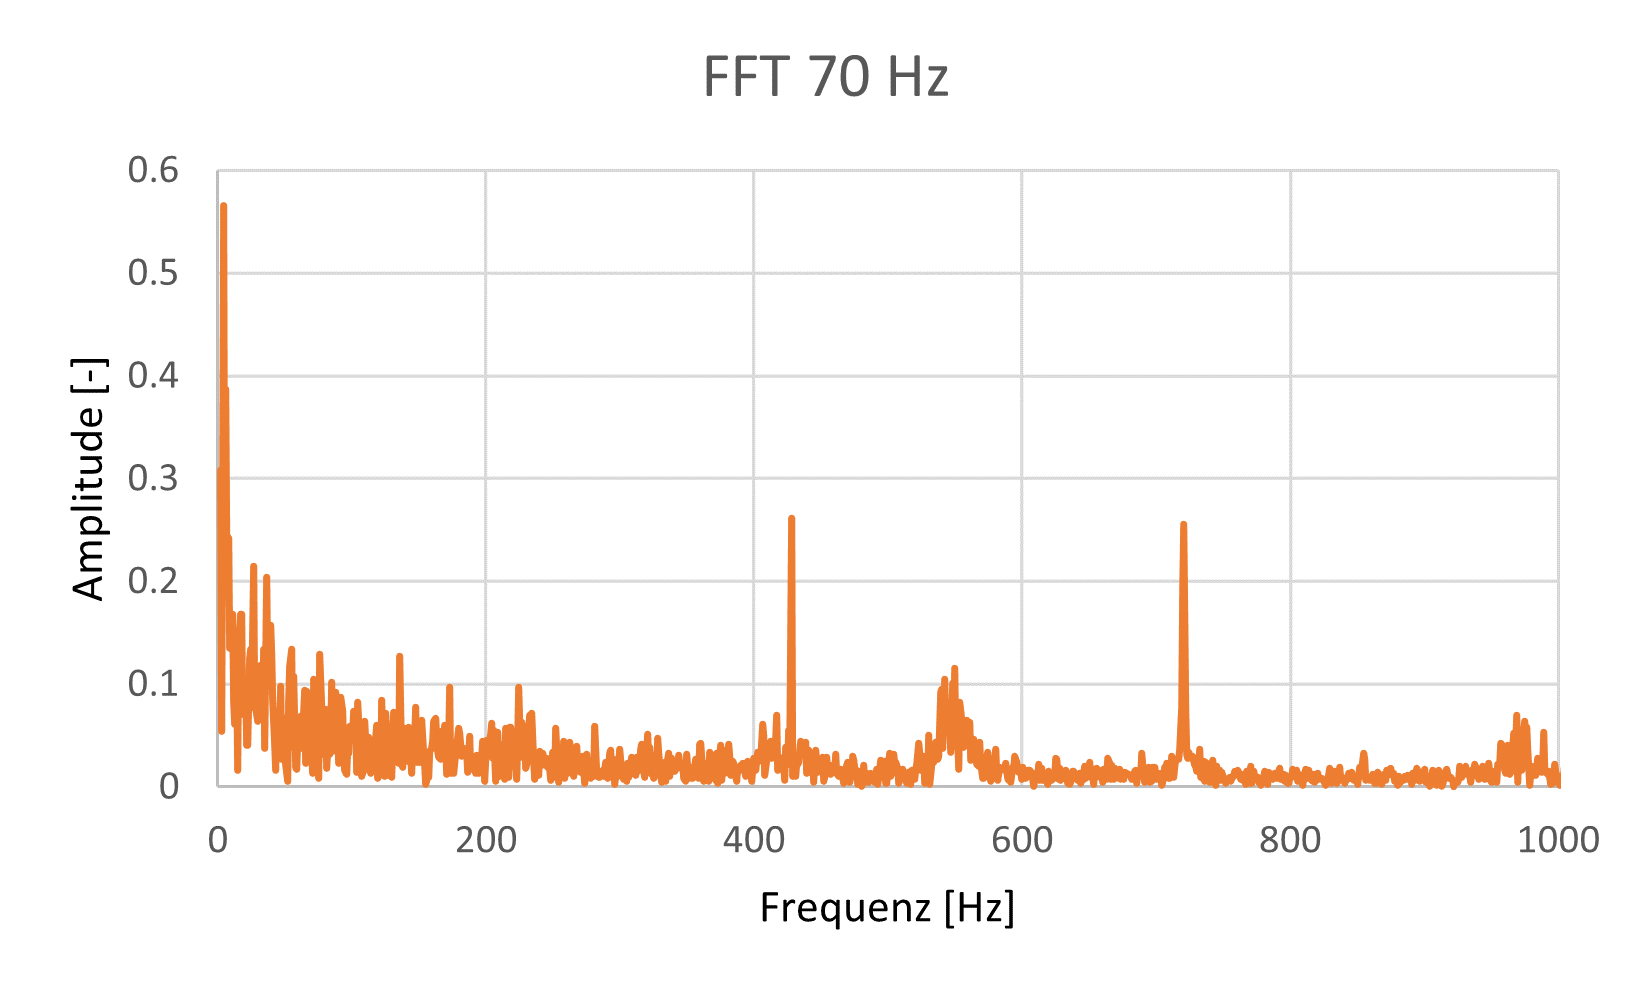
\includegraphics[width=1\linewidth]{imgs/FFT_70Hz}
	\caption{FFT 70 Hz Rauschen NP}
	\label{fig:fft70hz}
\end{figure}
\begin{figure}[H]
	\centering
	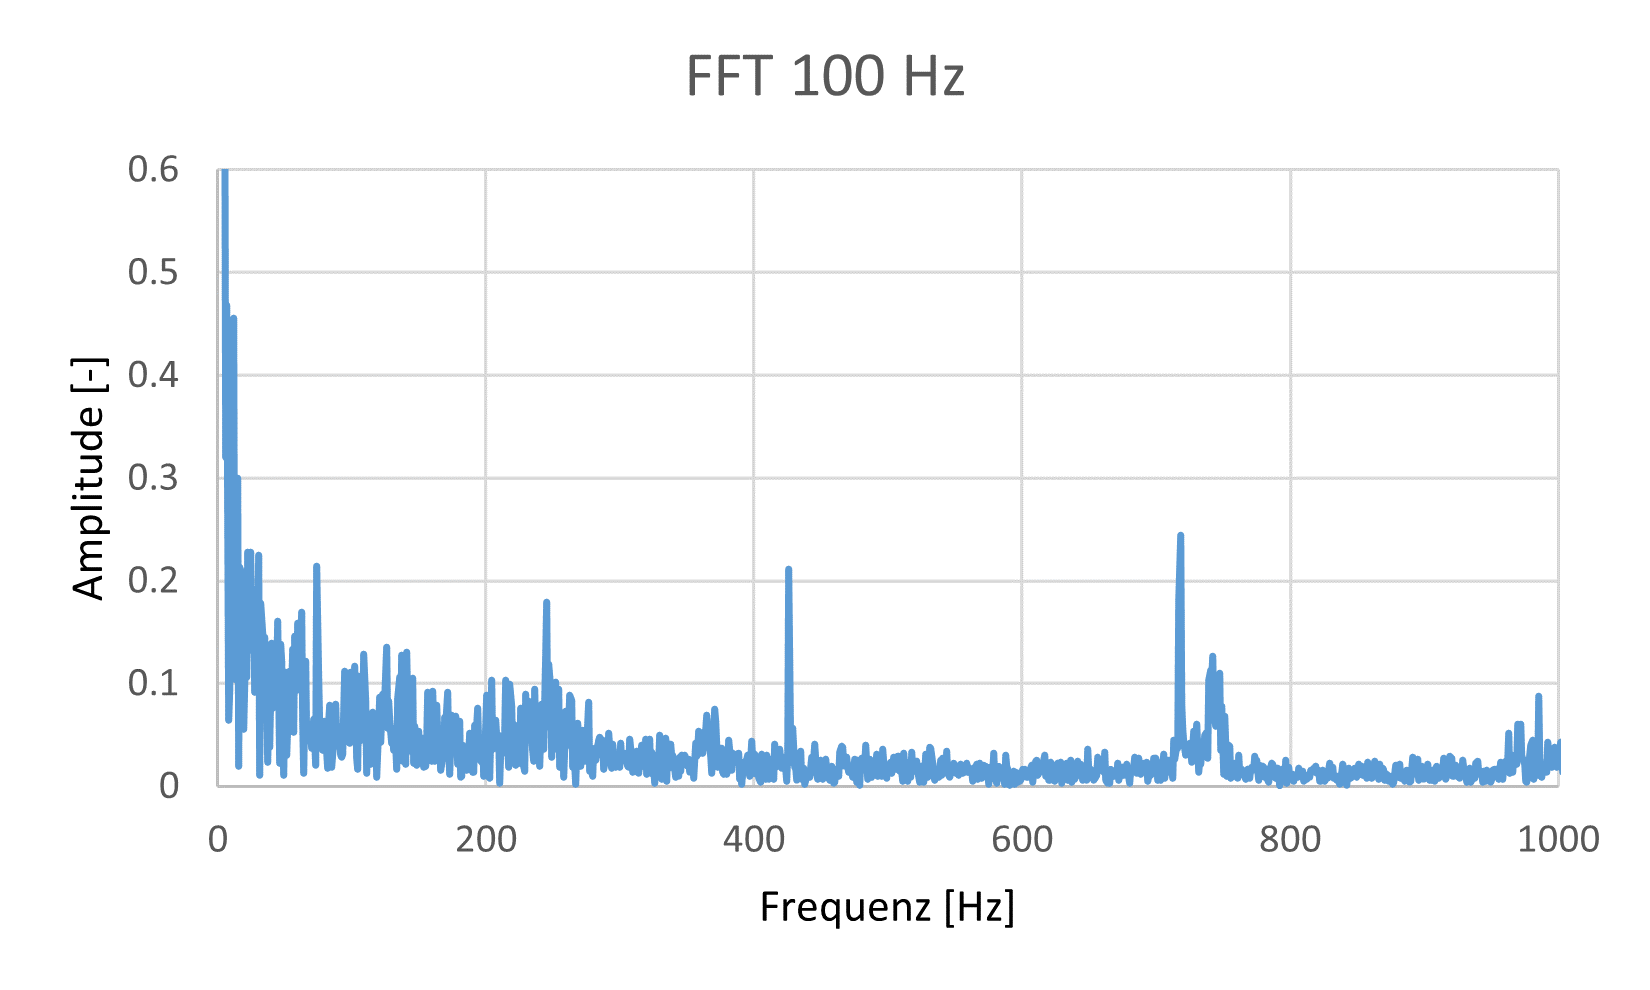
\includegraphics[width=1\linewidth]{imgs/FFT_100Hz}
	\caption{FFT 100Hz Rauschen Np}
	\label{fig:fft100hz}
\end{figure}
\begin{figure}[H]
	\centering
	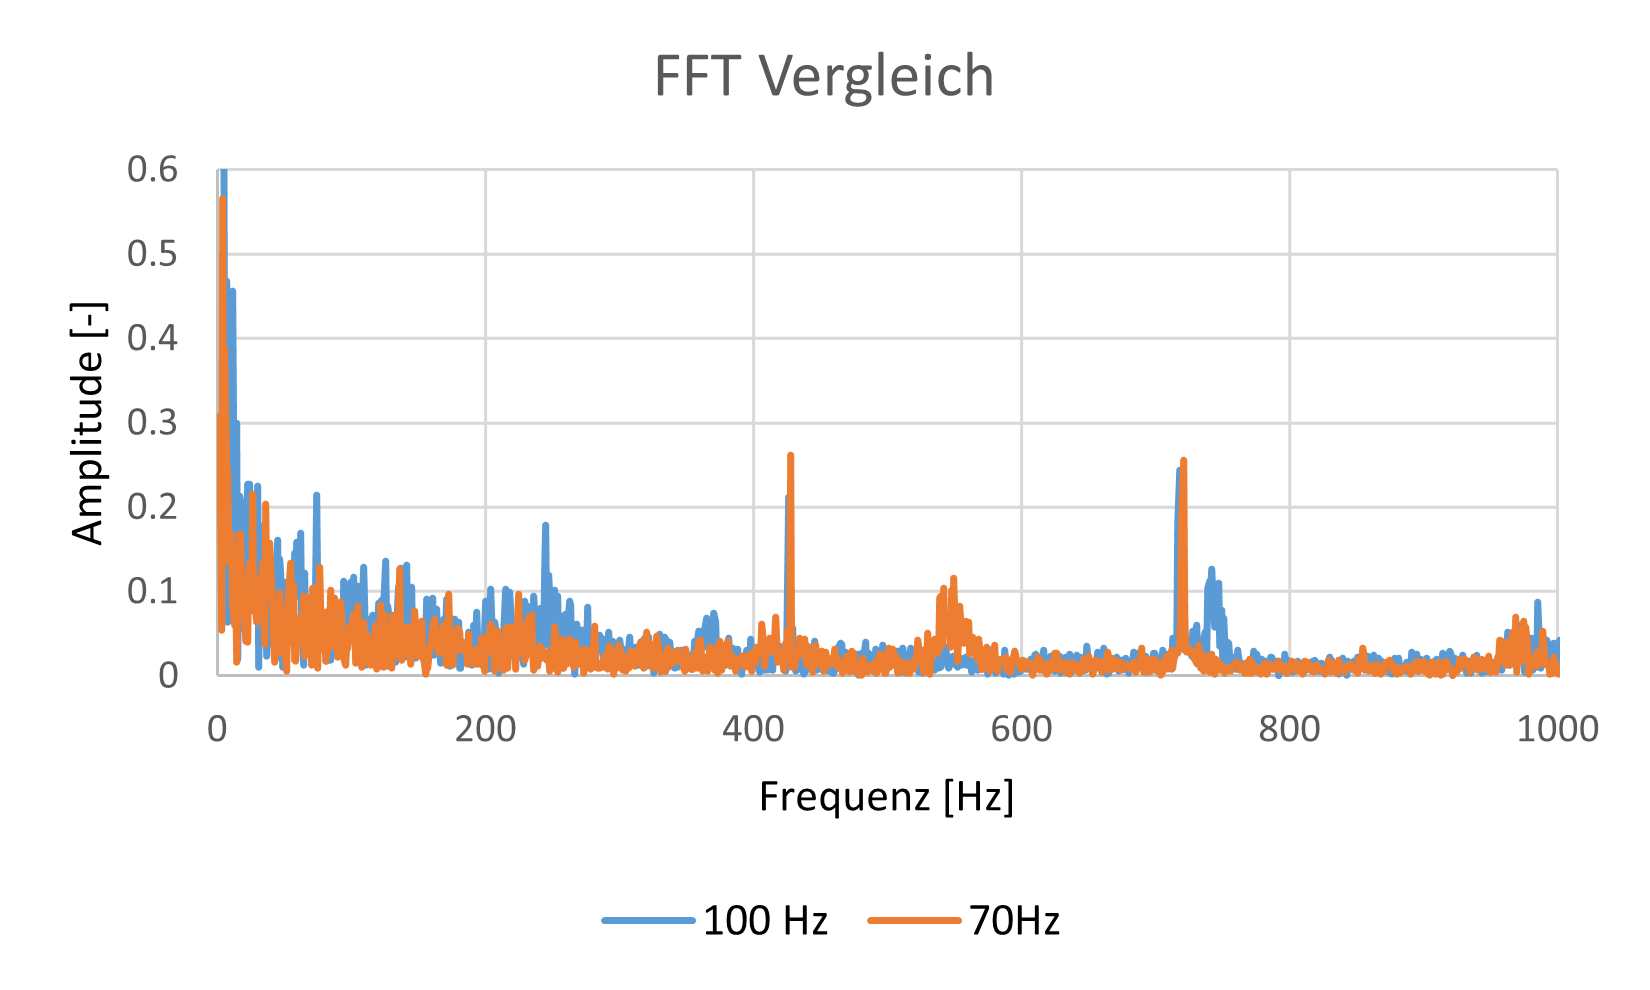
\includegraphics[width=1\linewidth]{imgs/FFT_Vergleich}
	\caption{FFT Vergleich}
	\label{fig:fftvergleich}
\end{figure}
Die Gegenüberstellung zeigt, dass das DuT mit Eckfrequenz 70 Hz im Allgemeinen alle Frequezanteile über 70 Hz stärker dämpft als jenes mit Eckfrequenz 100 Hz und erfüllt somit die Erwartungen. Auffallend ist jedoch, dass beide DuTs klare Peaks bei rund 440 und 720 Hz aufweisen.
\section{Langzeitbetrachtung Nullpunkt}
Aufgrund von Feedback aus der Fertigung bezüglich instabilen Nullpunkten sowie Beobachtungen aus Abbildung \ref{fig:vergleichlastverlauf} wurde der Nullpunkt der DuTs zusätzlich über einen Zeitraum von 10 Minuten aufgezeichnet. Die Messungen sind den Abbildung \ref{fig:np100long} und \ref{fig:np70long} zu entnehmen. Beide DuTs weisen einen deutlichen Nullpunktdrift von $\Delta S_{NP,100Hz}\approx 2\nicefrac{mV}{V}$ respektive $\Delta S_{NP,70Hz}\approx 1\nicefrac{mV}{V}$ auf
\begin{figure}[H]
	\centering
	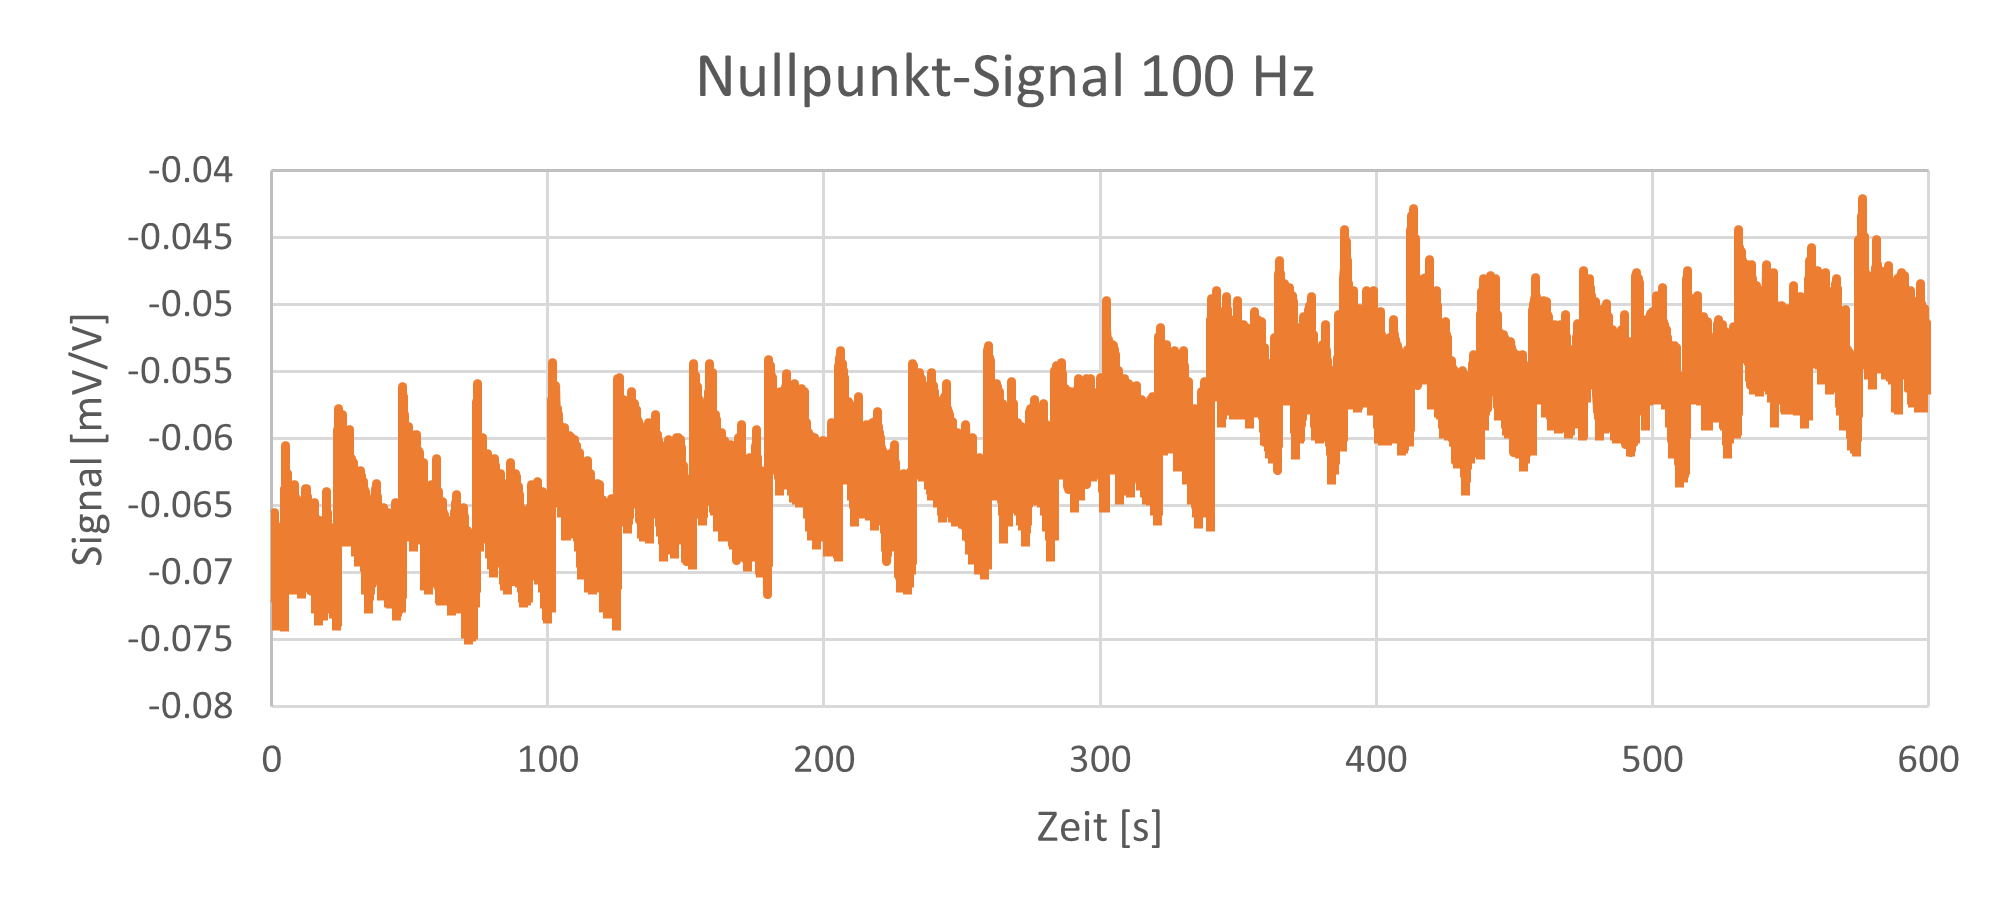
\includegraphics[width=1\linewidth]{imgs/NP100_Long}
	\caption{Nullpunkt-Verlauf 100Hz über 10min (600s)}
	\label{fig:np100long}
\end{figure}
\begin{figure}[H]
	\centering
	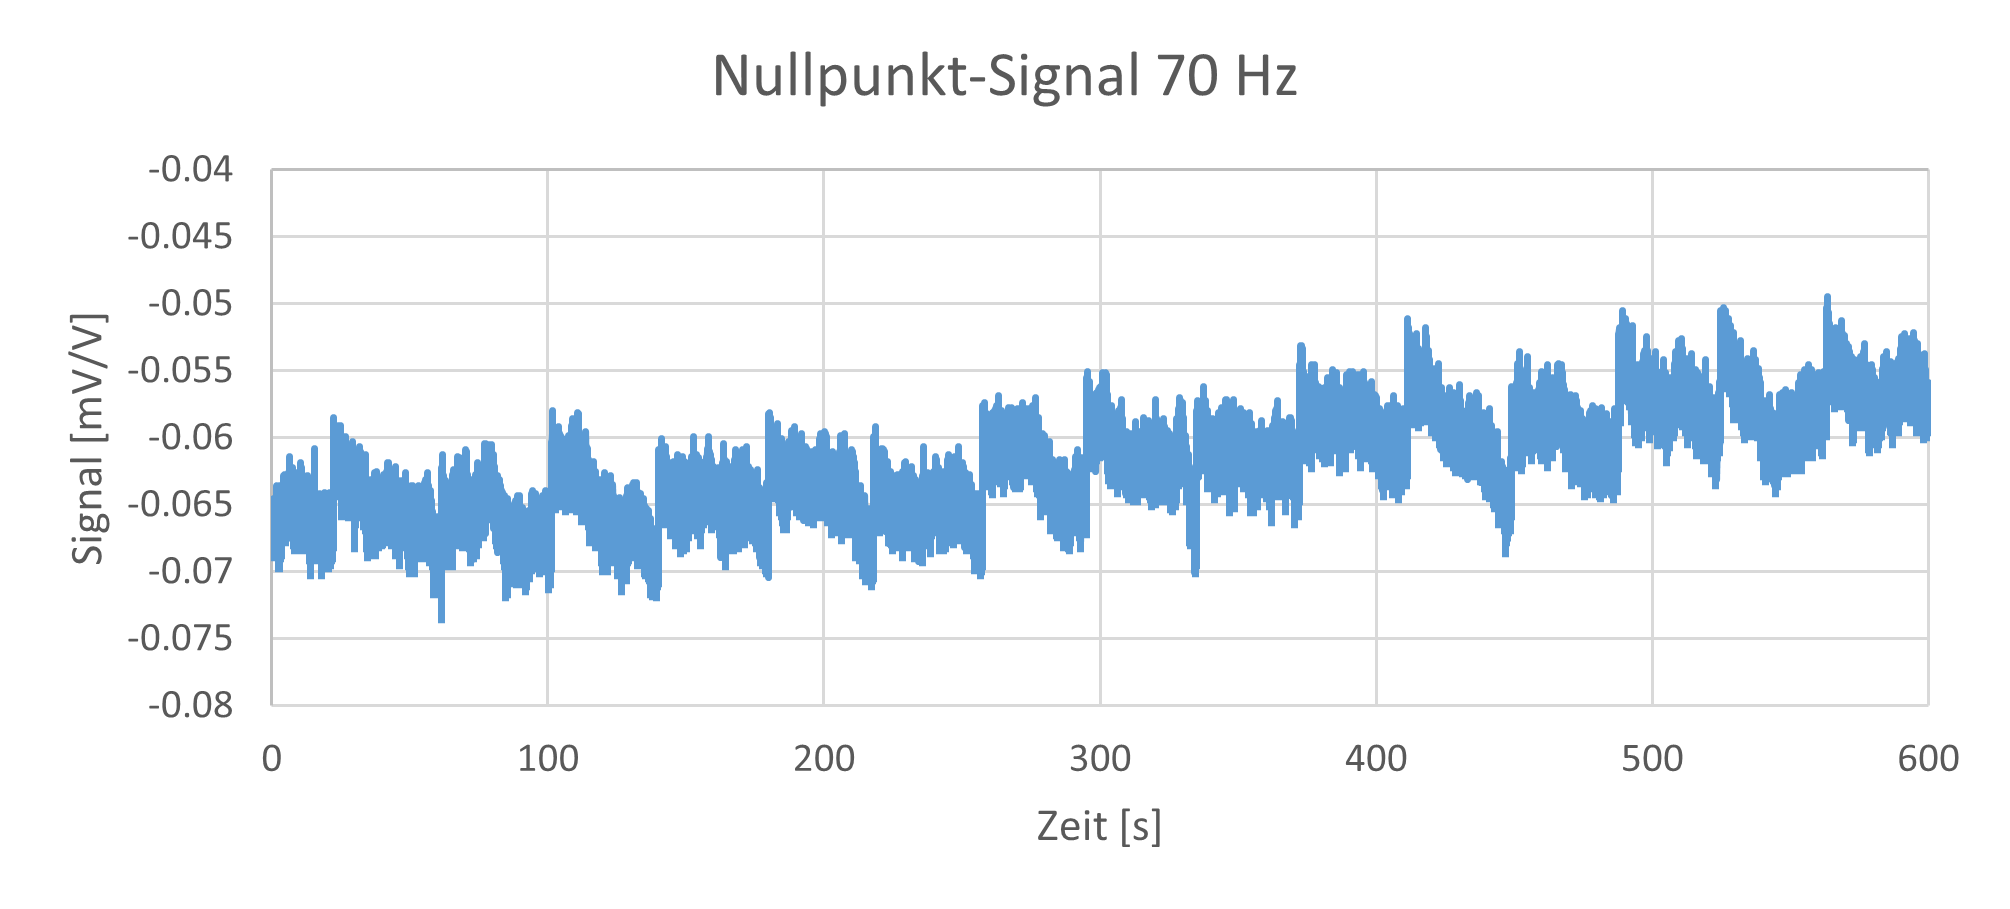
\includegraphics[width=1\linewidth]{imgs/NP70_Long}
	\caption{Nullpunkt-Verlauf 70Hz über 10min (600s)}
	\label{fig:np70long}
\end{figure}
Weiter zeigen die beiden obigen Messungen, dass der Nullpunkt periodisch springt. Dieser Effekt ist für den Zeitraum von 200 Sekunden (ab Sekunde 100) der obigen Messungen untenstehend nochmal dargestellt. Aus diesen Abbildungen kann eine Periodizität von $T_{NP, 100Hz} \approx 25s$ sowie $T_{NP, 70Hz} \approx 40s$ ermittelt werden. Innerhalb dieser Perioden fällt der Nullpunkt jeweils um rund $0.01 \nicefrac{mV}{V}$ ab, wobei das Signal über längere Zeiträume aufgrund der Sprünge insgesamt leicht steigt.
\begin{figure}[H]
	\centering
	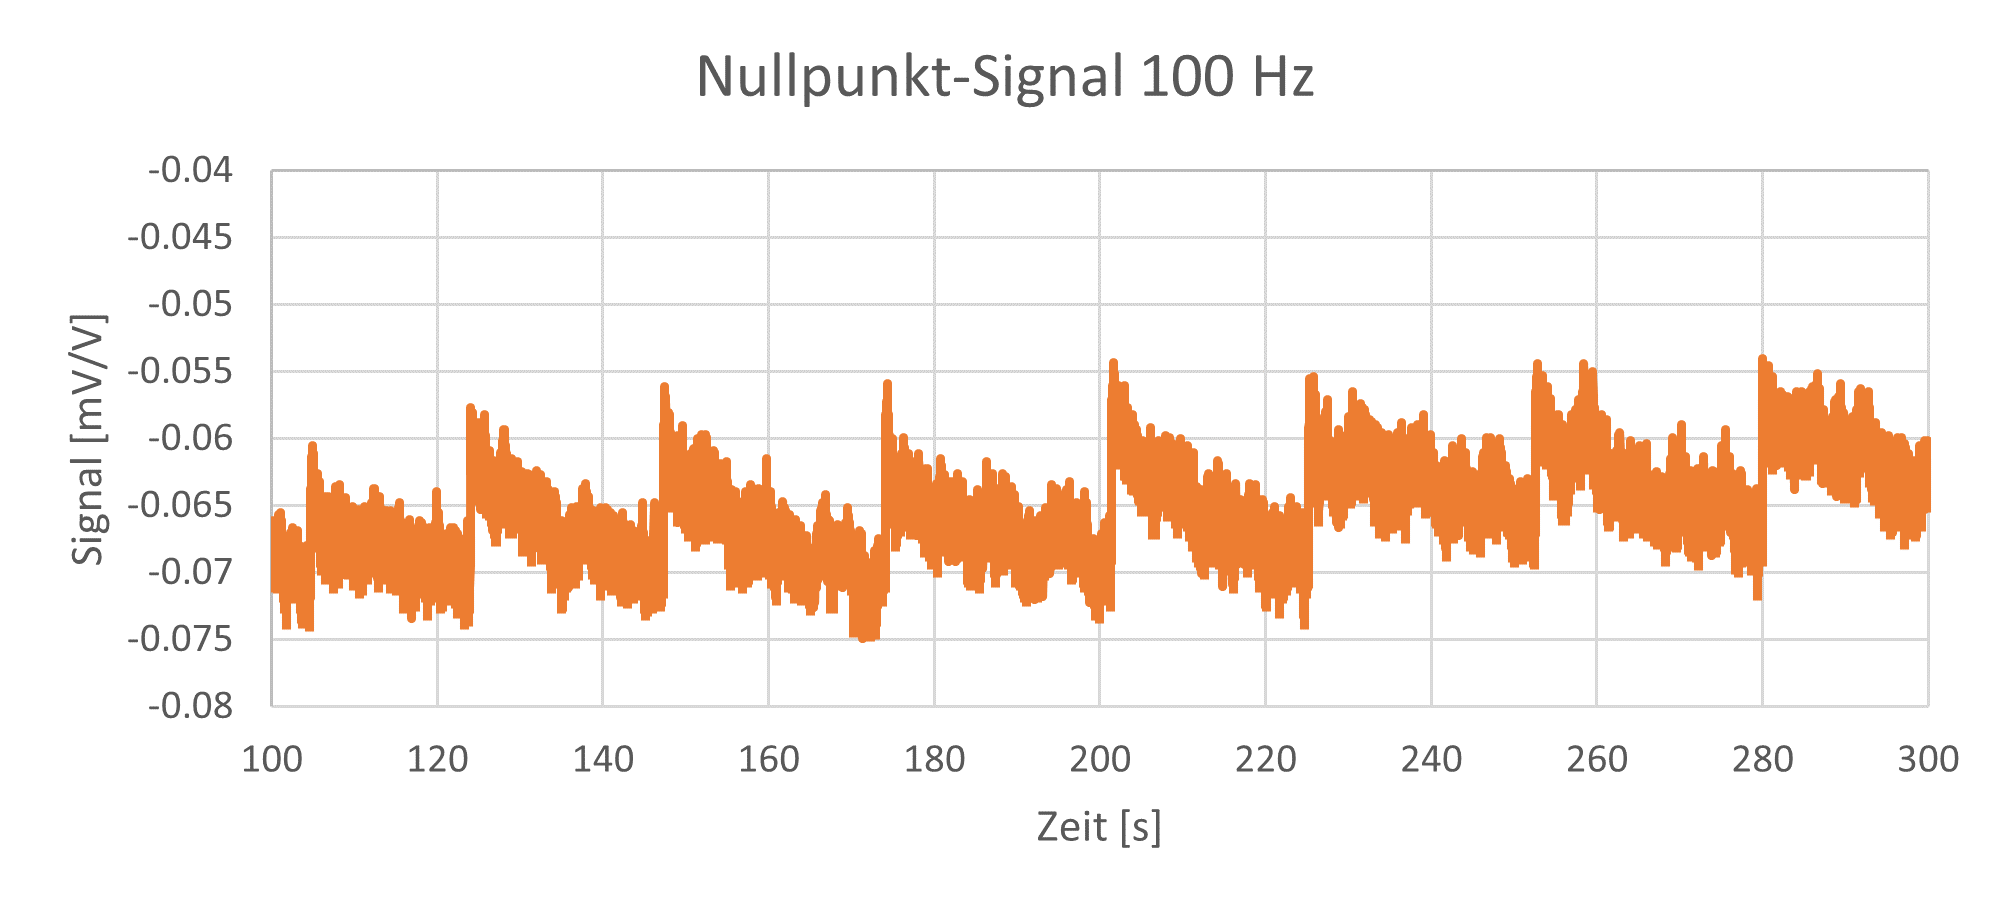
\includegraphics[width=1\linewidth]{imgs/NP100_SHORT}
	\caption{Nullpunkt-Verlauf 100Hz über 200s (Ausschnitt aus obigem Bild)}
	\label{fig:np100short}
\end{figure}
\begin{figure}[H]
	\centering
	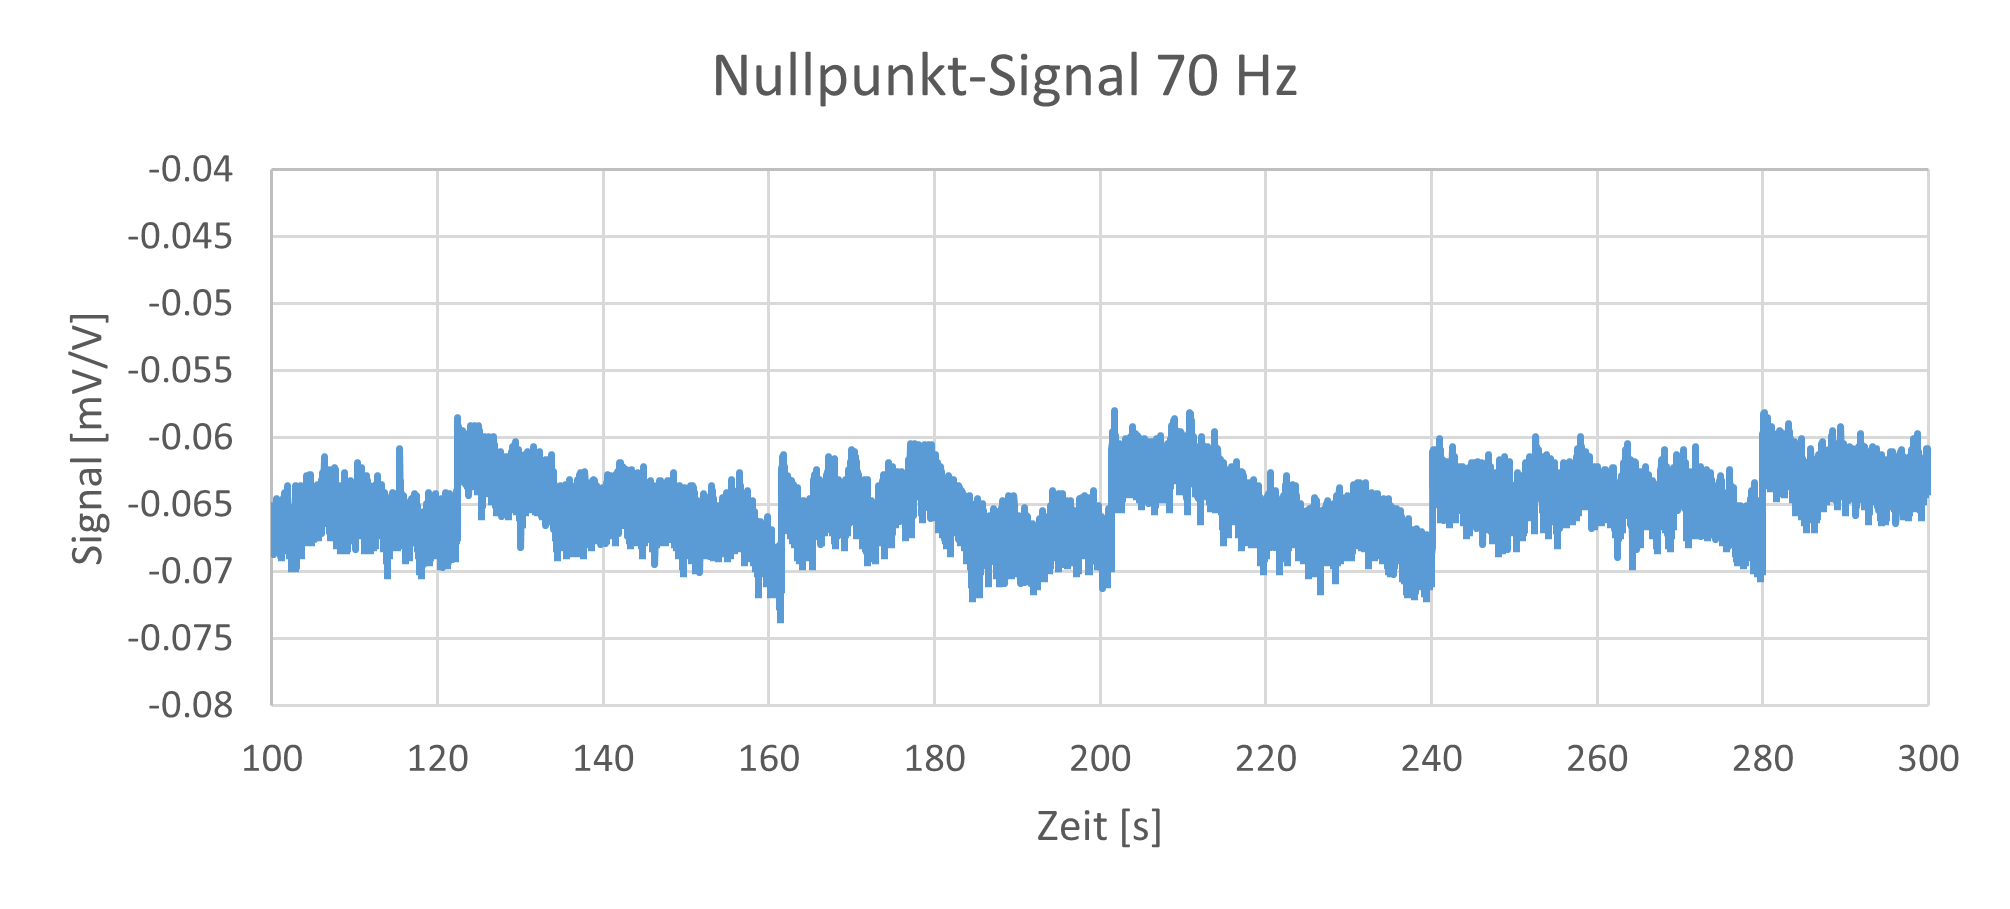
\includegraphics[width=1\linewidth]{imgs/NP70_SHORT}
	\caption{Nullpunkt-Verlauf 100Hz über 200s (Ausschnitt aus obigem Bild)}
	\label{fig:np70short}
\end{figure}
\section{Empfehlungen weiteres Vorgehen}
Um einen Messfehler auszuschließen, sollte die Messung allenfalls rasch reproduziert werden. Für diese Messungen wurde das Mess-Setup einige Stunden vor der eigentlichen Messung aufgebaut. Die  DuTs wurden permanent gespiesen und waren zum Zeitpunkt der Messung deutlich erwärmt. Im Falle einer Messwiederholung sollte daher gleich zu Beginn eine Messung durchgeführt werden (wenn die Sensorik / Elektronik noch kalt ist) und diese Messung dann nach einigen Stunden wiederholt werden. Aus diesem Ansatz könnten Erkenntnissen zum Aufwärmverhalten gewonnen werden. Weiter sollte die Software, welche auf den X-106-Prints läuft, überprüft werden. Eventuell kommt das periodische Springen der Nullpunkte auf der digitalen Seite des Signalprocessings zu Stande.
